\begin{figure}[!htp]
    \centering
    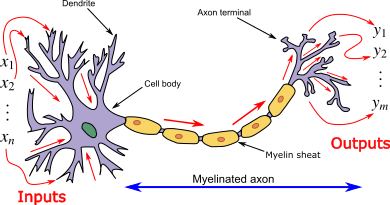
\includegraphics[width=10cm]{Images/neuron.png}
    \caption{Human neural structure}
    \label{figure:neuralStructure}
\end{figure}

The figure \ref{figure:neuralStructure} represents the biological structure of neurons that helps in the communication of electric signals in the nervous system to learn and process information. The biological structure of neurons
includes three major parts dendrites which are responsible for accepting the electrical and chemical signals to the neuron. 
Furthermore, the neuron contains the nucleus which is accountable for the processing input information with the neurons. 
At last, the processed information is passed to another neuron which is interconnected to neurons in the human nervous system through axon terminals
\citep{AGATONOVICKUSTRIN2000717}. 
